% Created 2021-09-20 Mon 08:08
% Intended LaTeX compiler: pdflatex
\documentclass[presentation,aspectratio=169]{beamer}
\usepackage[utf8]{inputenc}
\usepackage[T1]{fontenc}
\usepackage{graphicx}
\usepackage{grffile}
\usepackage{longtable}
\usepackage{wrapfig}
\usepackage{rotating}
\usepackage[normalem]{ulem}
\usepackage{amsmath}
\usepackage{textcomp}
\usepackage{amssymb}
\usepackage{capt-of}
\usepackage{hyperref}
\usepackage{amssymb}
\usepackage{circuitikz}
\usepackage{khpreamble}
\usepgfplotslibrary{groupplots}
\usetheme{default}
\author{Kjartan Halvorsen}
\date{\today}
\title{The DC motor}
\hypersetup{
 pdfauthor={Kjartan Halvorsen},
 pdftitle={The DC motor},
 pdfkeywords={},
 pdfsubject={},
 pdfcreator={Emacs 26.3 (Org mode 9.4.6)}, 
 pdflang={English}}
\begin{document}

\maketitle

\section{Intro}
\label{sec:org1ac59b1}

\section{The DC motor}
\label{sec:org49f77d8}
\begin{frame}[label={sec:orgf50b351}]{Force acting on an electric conductor in a magnetic field}
\begin{center}
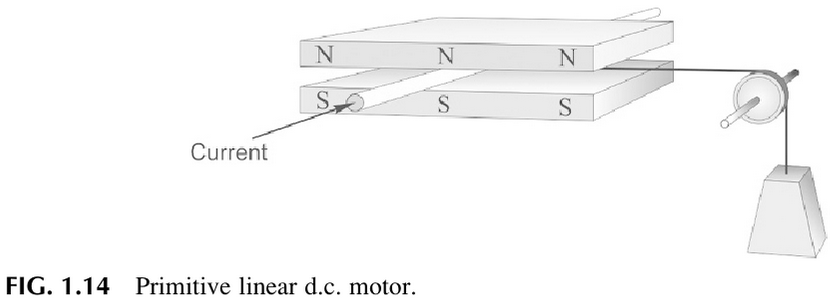
\includegraphics[width=0.4\linewidth]{../../figures/HD-fig1_14.png}
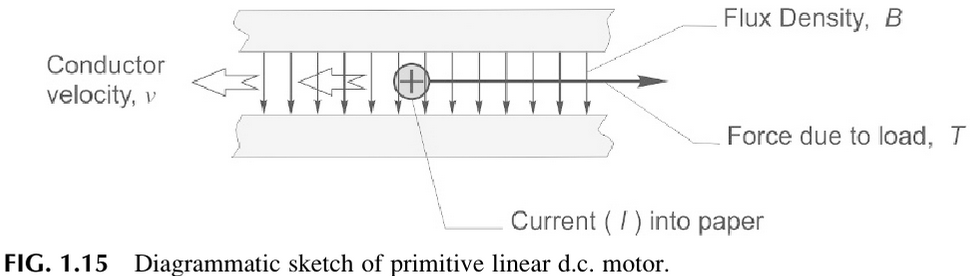
\includegraphics[width=0.53\linewidth]{../../figures/HD-fig1_15.png}
\footnotesize Source: Hughes and Drury ''Electric motors and drives''
\end{center}

\[F=k_mI=(Bl_m)I,\]
\end{frame}

\begin{frame}[label={sec:org479f6d4}]{Rotating motor}
\begin{center}
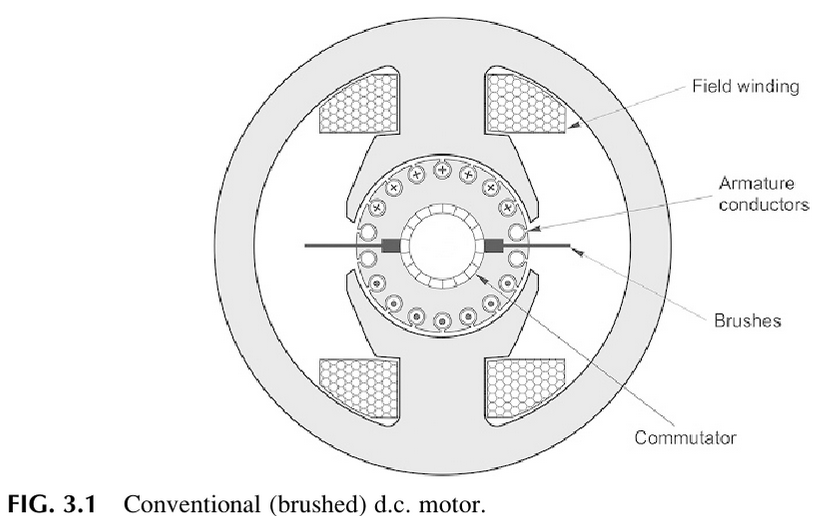
\includegraphics[width=0.4\linewidth]{../../figures/HD-fig3_1.png}
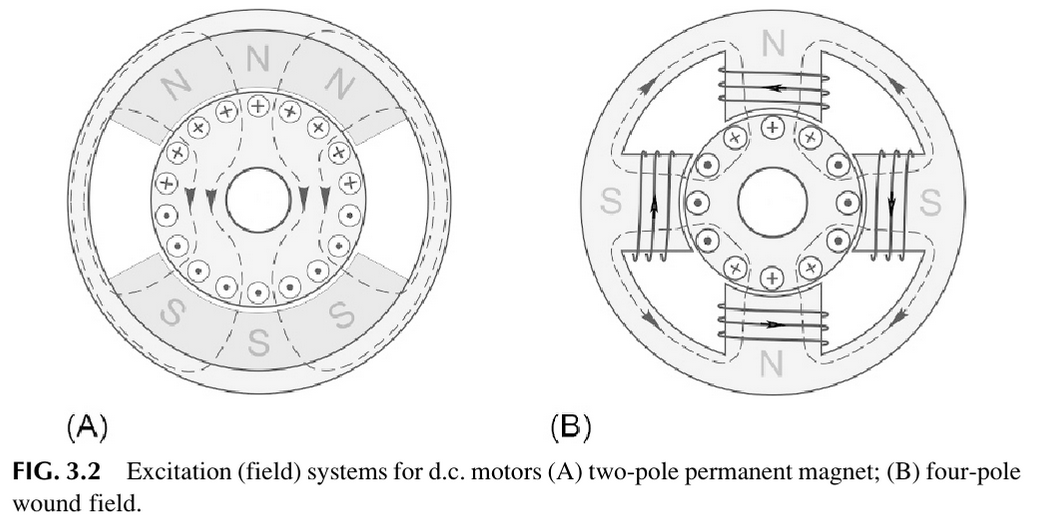
\includegraphics[width=0.53\linewidth]{../../figures/HD-fig3_2.png}
{\footnotesize Source: Hughes and Drury ''Electric motors and drives''}
\end{center}
\end{frame}

\begin{frame}[label={sec:org255a431}]{Magnetic force and electro-motive force}
\begin{block}{The magnetic force on a current-carrying conductor}
\[ F(t) = k_f i(t) \quad\Leftrightarrow\quad T(t) = k_f r i(t) = k_m i(t)\]
\end{block}

\begin{block}{Voltage generated in a conductor moving in a magnetic field}
\[ e(t) = k_v v(t) \quad\Leftrightarrow\quad e(t) = k_v r \omega(t) = k_e \omega(t)\]
\(e(t)\) is called  \emph{Back electro-motive force (Back e.m.f.)}.

\alert{In the SI-system units} \(k_m = k_e = k\).
\end{block}
\end{frame}

\begin{frame}[label={sec:orgf3a2f0f}]{Equivalent circuit}
Consider a DC motor with separate excitation
\begin{center}
  \begin{circuitikz}
    \draw (4,1) node[elmech](motor){M};
    \draw (motor.north) to[R=$R$] (4,4) to[L=$L$] (0,4)
    to[american voltage source, label=$u$] (0,0) -| (motor.south);
    \draw[thick,->>](motor.right)--++(1,0)node[midway,above]{$\omega$};

    \node[] at (2, -0.8 cm) {\(L \frac{d}{dt}i(t) +  Ri(t) + k\omega(t) = u\)};

    \node[] at (2, 4.5 cm) {Armature};

    \begin{scope}[xshift=8cm]
    \draw (0,1) to (4,1) to[R=$R_f$] (4,3) to[L=$L_f$] (0,3)
    to[american voltage source, label=$V_f$] (0,1);
    \node[] at (2, 4.5 cm) {Field};
    \end{scope}
  \end{circuitikz}
\end{center}

\begin{center}
Newton: \(J\frac{d}{dt}\omega(t) = ki(t) - T_l(t)\)
\end{center}
\end{frame}


\begin{frame}[label={sec:org25f647d}]{Modeling the DC motor}
\begin{center}
  \begin{circuitikz}[yscale = 0.5]
    \draw (4,2) node[elmech](motor){M};
    \draw (motor.north) to[short] (4,4) to[R=$R$] (2,4) to[L=$L$] (0,4)
    to[american voltage source, label=$u$] (0,0) -| (motor.south);
    \draw[thick,->>](motor.right)--++(1,0)node[midway,above]{$\omega$};

    \node[] at (9, 4 cm) {\(L \frac{d}{dt}i(t) +  Ri(t) + k\omega(t) = u\)};
    \node[] at (9, 2 cm) {\(\frac{d}{dt}i(t) = \frac{1}{L} \Big(-Ri(t) - k\omega(t) + u\Big)\)};
    \end{circuitikz}
    \end{center}
    \begin{center}
    \begin{circuitikz}[yscale = 1]
  \begin{scope}[xshift=8cm, yshift=-1cm,
  block/.style={rectangle, draw, minimum width=12mm, minimum height=10mm},
  amp/.style = {regular polygon, regular polygon sides=3,
        draw, fill=white, text width=1em,
        inner sep=1pt, outer sep=0mm,
        shape border rotate=-90},
	summ/.style = {circle, draw, inner sep = 1pt},]
   \node[block,] (int) at (0,0) {$\int$};
   \node[amp, left of=int, node distance=30mm] (oneoverL) {$\frac{1}{L}$}; 
   \draw[->] (oneoverL) -- node[above] {$\frac{d}{dt}i(t)$} (int);
   \node[summ, left of=oneoverL, node distance=20mm] (sum) {\small $\Sigma$};
   \node[coordinate, left of=sum, node distance=35mm] (Vin) {};
   \draw[->] (Vin) -- node[above, very near start] {$u$} node[coordinate, pos=0.6] (mp) {} (sum);
   \node[amp, above of=mp, node distance=15mm] (mkonst) {$-k$};
   \draw[->] (int) -- node[coordinate] (fb) {} node[above, near end] {$i(t)$} ++(25mm, 0);
   \draw[->] (mkonst) ++(-2cm, 0) -- node[above, near start] {$\omega(t)$} (mkonst);
   \draw[->] (mkonst) -| (sum);
   \draw[->] (sum) -- (oneoverL);
   \node[amp, below of =int, node distance=16mm, rotate=180] (RR) {\rotatebox{-180}{$-R$}};
   \draw[->] (fb) |- (RR) -| (sum);

   \end{scope}
  \end{circuitikz}
  \end{center}
\end{frame}


\begin{frame}[label={sec:org82727b0}]{Transmission}
\end{frame}

\begin{frame}[label={sec:org96d9455}]{Transmission}
  \begin{center}
  \begin{circuitikz}[xscale = 0.8]
\begin{scope}[xshift=8cm, yshift=-1cm,
block/.style={rectangle, draw, minimum width=12mm, minimum height=10mm},
amp/.style = {regular polygon, regular polygon sides=3,
      draw, fill=white, text width=1em,
      inner sep=1pt, outer sep=0mm,
      shape border rotate=-90},
      summ/.style = {circle, draw, inner sep = 1pt},]
 \node[block,] (int) at (0,0) {$\int$};
 \node[amp, left of=int, node distance=25mm] (oneoverL) {$\frac{1}{L}$}; 
 \draw[->] (oneoverL) -- node[above] {$\frac{d}{dt}i$} (int);
 \node[summ, left of=oneoverL, node distance=15mm] (sum) {\small $\Sigma$};
 \node[coordinate, left of=sum, node distance=45mm] (Vin) {};
 \draw[->] (Vin) -- node[above, very near start] {$u$} node[coordinate, pos=0.8] (mp) {} (sum);
 \node[amp, above of=mp, node distance=15mm] (mkonst) {$-k$};
 \node[amp, left of=mkonst, node distance=20mm] (gr) {$g_r$};
 \node[amp, right of=int, node distance=25mm] (mk2) {$k$};
 \node[amp, right of=mk2, node distance=20mm] (gr2) {$g_r$};
 \draw[->] (int) -- node[coordinate, pos=0.5] (meas) {} node[above] {$i$} (mk2);
 \draw[->] (mk2) -- node[above] {$T_m$} (gr2);
 \draw[->] (gr2) -- node[above] {$T_e$} ++(15mm, 0);
 \draw[->] (gr) ++(-2cm, 0) -- node[above, near start] {$\omega_a$} (gr);
 \draw[->] (gr) -- node[above, ] {$\omega_m$} (mkonst);
 \draw[->] (mkonst) -| (sum);
 \draw[->] (sum) -- (oneoverL);
 \node[amp, below of =int, node distance=16mm, rotate=180] (fb) {\rotatebox{-180}{$-R$}};
 \draw[->] (meas) |- (fb);
 \draw[->] (fb) -| (sum);
 \end{scope}
\end{circuitikz}
\end{center}

Ignoring losses in the transmission:
\[\underbrace{T_m\omega_m}_{\text{Power in}} = \underbrace{T_e\omega_a}_{\text{Power out}}\]
\end{frame}


\begin{frame}[label={sec:org7308dfa}]{DC motor driving a load}
  \begin{center}
  \begin{tikzpicture}[scale = 0.5,
block/.style={rectangle, draw, minimum width=12mm, minimum height=10mm},
amp/.style = {regular polygon, regular polygon sides=3,
      draw, fill=white, text width=1em,
      inner sep=1pt, outer sep=0mm,
      shape border rotate=-90},
      summ/.style = {circle, draw, inner sep = 1pt},]
 \node[block,] (dc) at (0,0) {$\frac{1/R}{s\frac{L}{R} + 1}$};
 \node[summ, left of=dc, node distance=20mm] (sum) {\small $\Sigma$};
 \node[coordinate, left of=sum, node distance=20mm] (Vin) {};
 \draw[->] (Vin) -- node[above, very near start] {$u$} node[coordinate, pos=0.8] (mp) {} (sum);
 \node[block, below of=sum, node distance=20mm] (mkonst) {$g_rk$};
 \node[block, right of=dc, node distance=25mm] (mk2) {$g_rk$};
 \node[summ, right of=mk2, node distance=20mm] (sumtorque) {\small $\Sigma$};
 \node[block, right of=sumtorque, node distance=20mm] (load) {$\frac{1}{Js}$};
 %\node[block, right of=load, node distance=25mm] (int) {$\frac{1}{s}$};
 \node[coordinate, right of = load, node distance=25mm] (output) {}; 
 \node[coordinate, above of = sumtorque, node distance=20mm] (tload) {}; 
 \draw[->] (sum) -- (dc);
 \draw[->] (dc) -- node[coordinate, pos=0.5] (meas) {} node[above] {$i$} (mk2);
 \draw[->] (mk2) -- node[above] {$T_a$} (sumtorque);
 \draw[->] (sumtorque) -- node[above] {} (load);
 \draw[->] (load)  -- node[coordinate,] (meas) node[above,] {$\omega_a$} (output);
 \draw[->] (mkonst) -- node[pos=0.9, left,] {$-$} (sum);
 %\draw[->] (int) --  node[very near end, above] {$\theta_a$} (output);
 \draw[->] (meas) |- (mkonst);
 \draw[->] (tload) -- node[right, very near start] {$T_l$} node [right, pos=0.9] {$-$} (sumtorque);
\end{tikzpicture}
\end{center}
\end{frame}





\begin{frame}[label={sec:org231c594}]{DC motor driving a load}
Assuming the inductance to be negligable.

  \begin{center}
  \begin{tikzpicture}[scale = 0.5,
block/.style={rectangle, draw, minimum width=12mm, minimum height=10mm},
amp/.style = {regular polygon, regular polygon sides=3,
      draw, fill=white, text width=1em,
      inner sep=1pt, outer sep=0mm,
      shape border rotate=-90},
      summ/.style = {circle, draw, inner sep = 1pt},]
 \node[block,] (dc) at (0,0) {$\frac{1}{R}$};
 \node[summ, left of=dc, node distance=20mm] (sum) {\small $\Sigma$};
 \node[coordinate, left of=sum, node distance=20mm] (Vin) {};
 \draw[->] (Vin) -- node[above, very near start] {$u$} node[coordinate, pos=0.8] (mp) {} (sum);
 \node[block, below of=sum, node distance=20mm] (mkonst) {$g_rk$};
 \node[block, right of=dc, node distance=25mm] (mk2) {$g_rk$};
 \node[summ, right of=mk2, node distance=20mm] (sumtorque) {\small $\Sigma$};
 \node[block, right of=sumtorque, node distance=20mm] (load) {$\frac{1}{Js}$};
 %\node[block, right of=load, node distance=25mm] (int) {$\frac{1}{s}$};
 \node[coordinate, right of = load, node distance=25mm] (output) {}; 
 \node[coordinate, above of = sumtorque, node distance=20mm] (tload) {}; 
 \draw[->] (sum) -- (dc);
 \draw[->] (dc) -- node[coordinate, pos=0.5] (meas) {} node[above] {$i$} (mk2);
 \draw[->] (mk2) -- node[above] {$T_a$} (sumtorque);
 \draw[->] (sumtorque) -- node[above] {} (load);
 \draw[->] (load)  -- node[coordinate,] (meas) node[above,] {$\omega_a$} (output);
 \draw[->] (mkonst) -- node[pos=0.9, left,] {$-$} (sum);
 %\draw[->] (int) --  node[very near end, above] {$\theta_a$} (output);
 \draw[->] (meas) |- (mkonst);
 \draw[->] (tload) -- node[right, very near start] {$T_l$} node [right, pos=0.9] {$-$} (sumtorque);
\end{tikzpicture}
\end{center}


\alert{Activity} What is the transfer function from the voltage input \(u(t)\) to the angular velocity \(\omega_a(t)\)?
\end{frame}



\begin{frame}[label={sec:orgacbd599}]{DC motor driving a load}
  \begin{center}
  \begin{tikzpicture}[scale = 0.5,
block/.style={rectangle, draw, minimum width=12mm, minimum height=10mm},
amp/.style = {regular polygon, regular polygon sides=3,
      draw, fill=white, text width=1em,
      inner sep=1pt, outer sep=0mm,
      shape border rotate=-90},
      summ/.style = {circle, draw, inner sep = 1pt},]
 \node[block,] (dc) at (0,0) {$\frac{k_1}{s\tau + 1}$};
 \node[summ, right of=dc, node distance=20mm] (sum) {\small $\Sigma$};
 \node[block, above of=sum, node distance=20mm] (loadtrf)  {$-\frac{k_2}{s\tau + 1}$};
 \node[coordinate, left of=dc, node distance=20mm] (Vin) {};
 \node[coordinate, above of=loadtrf, node distance=20mm] (tload) {};
 \node[coordinate, right of=sum, node distance=30mm] (output) {};

 \draw[->] (Vin) -- node[above, very near start] {$u$} node[coordinate, pos=0.8] (mp) {} (dc);
 \draw[->] (tload) -- node[right, very near start] {$T_l$} node [right, pos=0.9] {} (loadtrf);
 \draw[->] (dc) to (sum);
 \draw[->] (loadtrf) to (sum);
 \draw[->] (sum) -- node[above, near end,] {$\omega_a$} (output);

\end{tikzpicture}
\end{center}

\[ \tau=\frac{JR}{(g_rk)^2}, \quad k_1= \frac{1}{g_r k}, \quad k_2 = \textcolor{white}{\frac{R}{(g_r k)^2}} \]
\end{frame}
\end{document}